\chapter{Aufgabe 2}
\section{Speicherverwaltung und -zugriff}
Als faszinierendes Detail aus dem Zusammenspiel zwischen Betriebssystem und der Programmiersprache C habe ich mir die Speicherverwaltung und den Speicherzugriff ausgesucht. \par
Die Programmiersprache C erlaubt es Entwicklern direkt auf den Speicher zuzugreifen, diesen zu manipulieren und auf \textit{niedriger Ebene} zu verwalten.
Die Verwaltung auf niedriger Ebene bedeutet dass die Programmiersprache \textbf{direkten Zugriff} auf hardwarenahe Ressourcen hat ohne dafür Abstraktionen oder automatische Verwaltungsfunktionen zu benötigen.
Entwickler können den Speicher direkt manipulieren in dem sie Zeiger oder Speicheradressen im Programm verwenden. \par
C unterscheidet in Zwei Speicherbereiche.
Dem \textit{Heap} und dem \textbf{Stack}
Der Stack wird dafür verwendet lokale Variablen und Funktionsaufrufe zu verwalten.
Dieser wird nach dem Ende eines \textit{Scopes} automatisch destruiert. 
Der Heap erlaubt es Speicher während der Laufzeit des Programms zu reservieren und freizugeben und wird vom Entwickler verwaltet.
Dies kann die Effizienz und Flexibilität des C-Programms erhöhen.
Dort liegt allerdings auch die Gefahr.
Der Speicher wird nicht beim Verlassen des Scopes automatisch freigegeben.
Dies muss durch der Entwickler implementieren um Speicherlecks zu vermeiden. \par
Der Stack und der Heap werden gegeneinander zulaufend angelegt wie in Abbildung \ref{stackandheap} zu sehen ist.\cite{bökelmann:2023} \par

\begin{figure}[h]
	\centering
	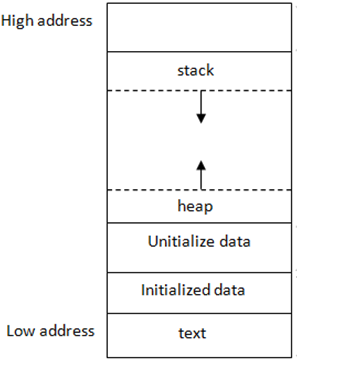
\includegraphics[scale=0.5]{Images/Speicher_layout.png}
	\caption{Schematische Anlegung des Stack und Heap\cite{stackandheap:2022}}
	\label{stackandheap}
\end{figure}

Dabei sollte darauf geachtet werden das in dem Fall das Stack und Heap immer größer werden, diese ineinander laufen und dies zur gegenseitigen Überschreibung der Daten führen kann. \par
Bei der Speicherverwaltung spielt ebenfalls das Betriebssystem eine wichtige Rolle.
Fordert ein C-Programm Speicher bei dem Betriebssystem an, interagiert diese mit dem Hardware-Speicher und reserviert einen Bereich im Speicher für das Programm.
Gibt das Programm den Speicher wieder frei, kann das Betriebssystem diesen recyclen und für andere Prozesse verwenden\cite{stackandheap:2022}. \par
Die Möglichkeit des Speicherzugriffs kann allerdings auch zu Sicherheitsproblemen führen.
Sicherheitslücken können entstehen wenn zum Beispiel mit Zeigern unvorsichtig umgegangen wird, die zu Pufferüberläufen führen.
Dies sollte vermieden werden und um Sicherheitsrisiken und potentielle Fehler zu minimieren\cite{bökelmann:2023}.

